\chapter{\label{background}Background on Bitcoin}
In this chapter, the necessary background information on the bitcoin protocol and the implementation of the client is presented. The focus lies on the parts of the protocol and the client that implement the peer-to-peer network.



\section{Primitives}
The fundamental task of the bitcoin protocol is to allow two arbitrary parties to exchange pieces of its currency, the bitcoins. The protocol calls the exchange of bitcoins a transaction.\\
The bitcoin protocol builds trust in an untrusted environment, it does so, by adding blocks of transactions to a global immutable distributed ledger, called blockchain. This chain is available on nodes participating in the bitcoin network. All transactions that are part of this chain can be verified by every protocol participant and this way, trust in the current state of the chain is generated. The protocol relys on the fact that no single authority controls this blockchain. In other words, no single authority is allowed to append to this chain at will. In bitcoin, this is ensured by the so called "proof-of-work". A mathematically hard problem must be solved in order to be allowed to add a block to the chain. This contains finding a nonce that when included to the input of a hash function, the resulting hash is below a certain threshold. There is no more efficient method to this mathematical riddle as the brute force trial-and-error approach. While finding a nonce which fulfils this requirement is hard, the verification of this proof-of-work is fast.  To generate an incentive for protocol participants to try to solve this task, the participant which finds a block receives an amount of bitcoins in form of a mix of a reward and of transaction fees from everyone performing a transaction. This procedure is generally known as "mining". The amount of people and the amount of computing power trying to solve these mathematical quizzes saw a continuous increase in the past 10 years. The protocol handles the automatic adaption of the threshold such that there is an expected delay of 10 minutes between two successive blocks. S.Nakamoto argues in \cite{nakamoto2008bitcoin} that such a distributed system prevents the double spending of bitcoins, if the majority of the computing work used to find a solution to the mathematical riddle is done by honest nodes.



\section{Peer-to-Peer protocol}
The bitcoin protocol describes a peer-to-peer network which is used to exchange transactions and blocks. Only the most important aspects of the protocol are sketched here. The interested reader is invited to read on in the bitcoin network documentation in \cite{bitcoinNetworkProtocol}.\\
A node in the bitcoin network maintains a given number of incoming (peer initiated) and outgoing (self initiated) connections to other peers. Using these connections, the node is able to receive and distribute transactions and blocks. Transactions are exchanged using a mix of advertisement and request: nodes will regularly send inventory (inv) messages to their peers containing identifying hashes of new transactions. The peer can check, which transactions it does not currently have and requests them from the peer it received the inv message from. Only then, this peer sends the whole transaction.\\
Using headers messages, the nodes regularly exchange their view on the blockchain. If a node notices, that a peer has a block which itself does not know, it requests the block using a compact block (cmpctblk) message. The peer will then respond with the compact block which contains the block header and a list of transactions that belong to this block. The traditional approach in exchanging blocks was to use the same mechanism as for exchanging transactions. In the second approach, the block is transmitted as a whole while in the first approach, the block is reconstructed at the receiver using the knowledge about the transactions it already possesses. As the legacy way of exchanging messages causes larger message sizes and needs longer to be verified, the compact block is preferred and commonly used. However, the traditional approach is used when the other end of the connection is too far behind the current head of the chain as it is improbable that the peer already has transactions belonging to a specific block.\\
Ping and pong messages are another message type. To test connectivity and measure the latency to its peers, a node regularly initiates ping messages to which the peer has to respond with pong messages.\\
The peer-to-peer network protocol allows different other message types which are not important for this work. The documentation for all message types in the current version of the bitcoin client can be found in \cite{bitcoinNetworkProtocol}.


\section{Client structure}
To understand the changes made to the bitcoin client, it is important to have a basic understanding of the implementation of the bitcoin client. The focus of this piece of background information lies on the peer-to-peer network part of version 0.16 of the bitcoin client. The client is multithreaded and the structure that it uses can be used to explain the logical structure of the program. We lay the focus on two threads. The first one is referred to as the SocketHandler thread. This part of the client is responsible handling incoming and outgoing messages. The second one is referred to as MessageHandler thread, which is responsible for processing the incoming messages and to assemble outgoing messages.\\
We start the explanation with an overview of the message processing pipeline that can be found in the bitcoin client. The explanation will use figure \ref{fig:dataflow} as illustration of the path of the messages in the system. The following paragraph includes numbers which link to the individual parts of this illustration. Per connection, the client maintains a data structure called CNode. This CNode is shared between the SocketHandler and the MessageHandler. The client also maintains one socket structure per client. Incoming messages are waiting in the sockets to be read. The SocketHandler regularly checks all sockets for new packets (1). If there are new packets, they are read from the socket and added to a message queue in the shared state between the SocketHandler and the SocketHandler (2). A message can consist of many packets. As soon as one message is finished, a signal is sent to the MessageHandler which reads the message from the CNode (3). The MessageHandler checks the consistency of the message and analyses its payload. According to the message type, different tasks are then performed. For example, transactions and blocks are verified and stored or the local storage is checked for transactions mentioned in advertisements. Finally, the MessageHandler assembles the reply to the peer. If possible, this message is then immediately sent by the MessageHandler (4). If this is not possible, the response is written to the CNode and the SocketHandler is informed that there is a new outgoing message waiting (5). The SocketHandler regularly checks the CNodes for outgoing messages and sends them to the corresponding peer (6).\\
There is a large amount of shared information between the SocketHandler and the MessageHandler. There is a list of CNodes and there are the CNodes themselves. To prevent access race conditions and keep the state consistent, they are protected using mutexes. Write and read accesses to individual parts of the CNodes require acquiring a lock.

\begin{figure}[!htb]
	\begin{center}
		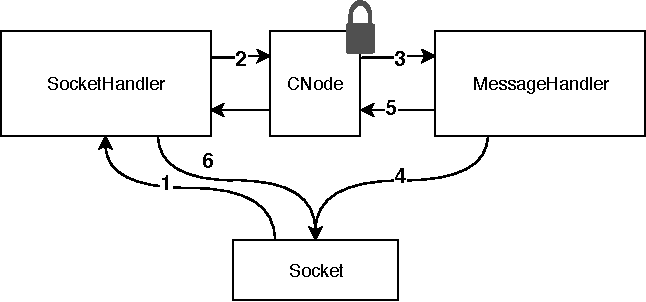
\includegraphics{Figures/dataflow}
		\caption[Overview of the message handling process in the bitcoin client.]{\label{fig:dataflow} Overview of the message handling process in the bitcoin client. This figure illustrates the flow of a message through the networking part of the bitcoin client.}
	\end{center}
\end{figure}



%\section{\label{background:scaling} Scaling issues}
%FDsets, Mutex, etc. refer to chapter on profiling




